\documentclass[dwyatte_dissertation.tex]{subfiles} 
\begin{document}

\sloppy

\chapter{Effects of spatial and temporal prediction during prolonged learning of novel objects}
\label{chap:bpleast}

\section{Introduction}
The core challenge of object recognition is concerned with solving the invariance problem \cite{DicarloZoccolanRust12}. Essentially, object identity must remain invariant across large changes in a an object's visual position, scale, rotation, and viewpoint to generate successful behavior. Understanding how exactly the brain solves this problem has been a major focus of the object recognition literature with the bulk of data and models suggesting that it is solved gradually by a hierarchy of neural processing mechanisms from V1 through inferior temporal (IT) cortex that extract increasingly complex features at each stage with increasing tolerance to transformations \cite{Fukushima80,RiesenhuberPoggio99,WallisRolls97,MasquelierThorpe07,OReillyWyatteHerdEtAl13}.

One question that remains to be fully answered is how the synaptic projections that support invariance are learned in the first place. One intriguing hypothesis is that a temporal association rule might form associations between multiple samples of a single object as it undergoes transformations \cite{StringerPerryRollsEtAl06,WallisBaddeley97,IsikLeiboPoggio12}. It has been demonstrated that some neurons can form temporal associations between arbitrary pairs of stimuli \cite{SakaiMiyashita91}, including a population in monkey IT cortex \cite{MeyerOlson11}. Experiments by DiCarlo and colleagues have indicated that these temporal associations can build new invariance for specific object transformations including changes in position and size \cite{CoxMeierOerteltEtAl05,LiDiCarlo08,LiDiCarlo10}. This new invariance can be learned without supervised reward, suggesting that it could be a natural consequence of generic neural processing mechanisms given the spatiotemporal statistics of the physical world \cite{LiDiCarlo12}.

Evidence of invariance due to temporal association has yet to be demonstrated in IT neurons for three-dimensional changes in viewpoint \cite[although see][for relevant human behavioral work]{WallisBulthoff01,WallisBackusLangerEtAl09}. IT neurons typically have a tuning curve of approximately 90 degrees for three-dimensional objects \cite{LogothetisPaulsBulthoffEtAl94,LogothetisPaulsPoggio95}, but these objects can be recognized irrespective of viewpoint after prolonged exposure \cite{WallisBulthoff99,EdelmanBulthoff92,TarrGauthier98}. Intuitively, predictable motion from one moment to the next could be considered important for encoding three-dimensional structure \cite{LawsonHumphreysWatson94,Stone98,VuongTarr04,BalasSinha09b,BalasSinha09c,ChuangVuongBulthoff12}, and thus a temporal association rule could plausibly be used to group together multiple viewpoints from naturalistic spatial structure of objects.

The work described in this chapter investigated the role of predictable spatiotemporal information during a novel object learning task. In the context of the LeabraTI model (Chapter \ref{chap:leabrati}) as well as several other theories of sensory prediction \cite{ArnalGiraud12,GiraudPoeppel12}, spatial structure might be learned from predictions about incoming sensory information made at regular temporal intervals. To test this hypothesis, both the spatial and temporal predictability of changes in objects' viewpoint were manipulated during a training period followed by a series of same-different judgements over static test views.

Somewhat surprisingly, the results of the experiment indicated that accuracy was lowest when stimuli were learned in a combined spatially and temporally predictable context and highest when learned in a completely unpredictable context. Reaction times were also slower when objects were learned with spatial predictability.

\section{Methods}

\subsection{Participants}
A total of 62 students from the University of Colorado Boulder participated in the experiment (ages 18-22, mean=19.11 years; 30 male, 32 female). All participants reported normal or corrected-to-normal vision and received course credit as	compensation for their participation. Informed consent was obtained from each participant prior to the experiment in accordance with Institutional Review Board policy at the University of Colorado.

\subsection{Stimuli}
Novel ``paper clip'' objects similar to those used in previous investigations of three-dimensional object recognition \cite{BulthoffEdelman92,EdelmanBulthoff92,LogothetisPaulsBulthoffEtAl94,LogothetisPaulsPoggio95,SinhaPoggio96} were used as stimuli (see Chapter \ref{chap:pleast} Methods). A total of eight objects were used -- four as targets and four as distractors. The four target objects were also used in the Chapter \ref{chap:pleast} experiment. Target and distractor objects were paired together for the purposes of the experiment. All objects are shown in Figure \ref{fig:bpleast_objs}.

% paperclip targets fig
\begin{figure}[h!]
\textbf{A} \\
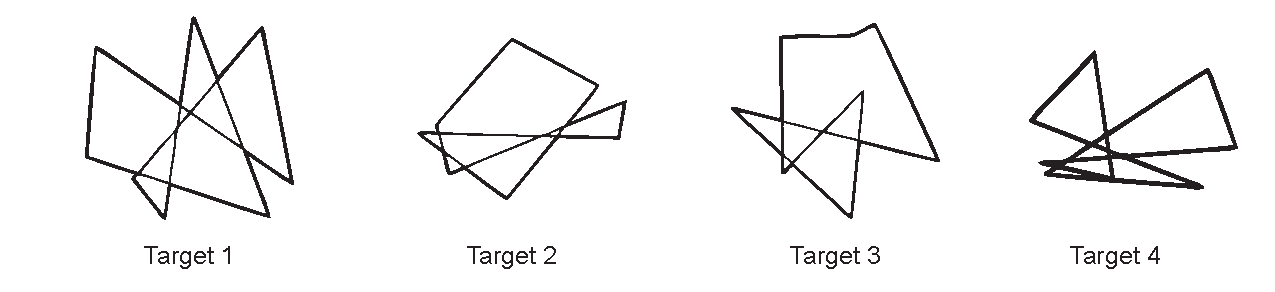
\includegraphics[width=160mm]{figs/chap_bpleast/paperclip_targets.pdf} \\
\textbf{B} \\
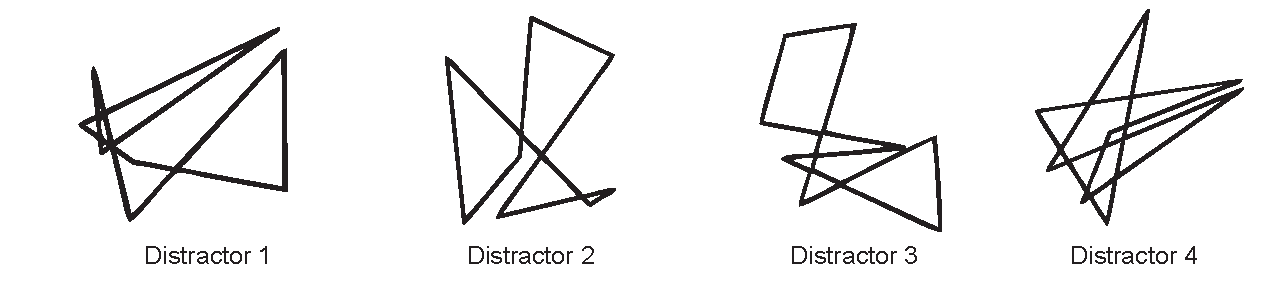
\includegraphics[width=160mm]{figs/chap_bpleast/paperclip_distractors.pdf} \\
\caption{Novel ``paper clip'' objects}{Four target (\textbf{A}) and four distractor object pairs (\textbf{B}) used in the experiment. See Chapter \ref{chap:pleast} Methods for additional information.}
\label{fig:bpleast_objs}
\end{figure}

\subsection{Procedure}
The experiment was divided into 16 blocks, each containing a training period followed by a series of test trials (Figure \ref{fig:bpleast_task}). During the training period of a given block, participants observed one of the target objects rotate about its y-axis. The object either rotated coherently (i.e., spatially predictable, S+ conditions) or in a random manner (S- conditions). Coherent rotation was composed of adjacent views spaced 12 degrees apart. The object made four complete rotations during the study period. All views of the object were still presented four times each in the random case. The presentation rate during the study period was either 10 Hz with a 50 ms on time and 50 ms off time (i.e., temporally predictable, T+ conditions) or variable with a 50 ms on time and off times ranging from 17-400 ms (T- conditions). 

The S+/- and T+/- conditions were crossed and each of the target-distractor object pairs was assigned to one of the four conditions. These assignments were approximately counterbalanced across participants (Assignment 1: \textit{N}=15; Assignment 2: \textit{N}=17; Assignment 3: \textit{N}=15; Assignment 4: \textit{N}=15). Each block condition with its target-distractor pairing was repeated for four blocks during the experiment. Block order was randomized for each participant.

During each block, participants were instructed to study the target object during the training period and then complete a series of 30 test trials. On each test trial, either the target object or its paired distractor was presented. Participants were instructed to respond ``same'' if they believed the object depicted the trained target object or ``different'' if they believed it depicted the distractor object. Half of the test trials contained 15 views of the target object spaced 24 degrees apart, and the other half contained 15 views of the distractor, also spaced 24 degrees apart. Test trials were shown in a random order and feedback was withheld to prevent participants from changing their response criteria over the course of a block. 

The experiment was displayed on an LCD monitor at native resolution operating at 60 Hz using the Psychophysics Toolbox Version 3 \cite{Brainard97,Pelli97}. All stimuli were presented at central fixation on an isoluminant 50\% gray background and subtended approximately 5 degrees of visual angle. Test trials began with a fixation cross (200 ms) followed by a blank (400 ms) followed by the probe stimulus (100 ms). Participants were required to respond within 2000 ms or the trial was aborted. Subsequent test trials were separated by a variable intertrial interval of 1000-1400 ms.

The experiment began with a practice block to ensure that participants understood the task that was later discarded from analysis. The training period during the practice block was always spatially and temporally predictable and used a reserved target object and distractor that were not further used in any of the experimental blocks. During the practice test trials, participants received feedback after responding according to whether they were correct or incorrect. After completing the practice block, participants were informed that future training periods could be presented in spatially and/or temporally unpredictable manners.

% paperclip targets fig
\begin{figure}[h!]
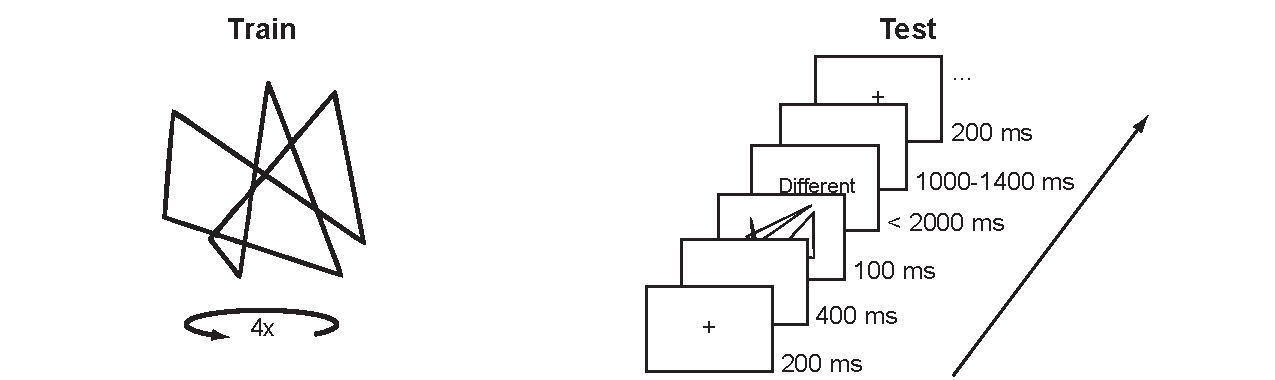
\includegraphics[width=160mm]{figs/chap_bpleast/paperclip_task.pdf} \\
\caption{Experimental procedure}{Experimental trials were composed of a training period followed by a testing period. The training period depicted a target object rotating a total of four times around its vertical axis. Rotation was either spatially and temporally predictable, spatially predictable or temporally predictable only, or completely unpredictable. The test period contained 30 trials that depicted either the training object or its paired distractor at 15 viewing angles each.}
\label{fig:bpleast_task}
\end{figure}

\section{Results}
Three subjects were excluded from behavioral analysis for accuracy 2.7$\sigma$ (or further) below mean accuracy across subjects. All three excluded subjects were assigned condition-object 3 resulting in the final counterbalancing -- Assignment 1: \textit{N}=15; Assignment 2: \textit{N}=14; Assignment 3: \textit{N}=15; Assignment 4: \textit{N}=15. The resulting 59 subjects were submitted to a 2x2 ANOVA with spatial and temporal predictability as within-subjects factors and counterbalancing assignment as a between-subjects factor. Accuracy and reaction times were collected during the experiment and were used to compute \textit{d'}, a measure of sensitivity that takes into account response bias, and inverse efficiency, a measure that combines accuracy and reaction times \cite{TownshendAshby78,TownshendAshby83}. These behavioral measures are plotted in Figure \ref{fig:bpleast_behave}.

% oh, behave
\begin{figure}[h!]
\begin{center}
\begin{tabular}{ll}
\includegraphics[width=80mm]{figs/chap_bpleast/results_accuracy.pdf} & 
\includegraphics[width=80mm]{figs/chap_bpleast/results_dprime.pdf} \\
\includegraphics[width=80mm]{figs/chap_bpleast/results_rt.pdf} &
\includegraphics[width=80mm]{figs/chap_bpleast/results_ie.pdf} \\
\end{tabular}
\end{center}
\caption{Behavioral measures of spatial and temporal predictability}{Accuracy, \textit{d'} (sensitivity), reaction time, and inverse efficiency (reaction time divided by percent correct) as a function of predictability during the training period. S-/+ refers to spatially unpredictable and predictable, T-/+ to temporally unpredictable and predictable. Error bars depict within-subjects error using the method described in \protect\incite{Cousineau05} adapted for standard error.}
\label{fig:bpleast_behave}
\end{figure}

% Acc
% Assignment: F(1, 57) = 0.156, p = 0.694
% Spatial: F(1, 57) = 4.496, p = 0.0383 * 
% Temporal: F(1, 57) = 4.149, p = 0.0463 * 
% Int: F(1, 57) = 0.197, p = 0.659

Overall, subjects were less accurate when the training period was spatially predictable (\textit{F}(1, 57) = 4.50, \textit{p} = 0.038) or temporally predictable (\textit{F}(1, 57) = 4.20, \textit{p} = 0.046). The interaction between spatial and temporal predicability failed to reach significance (\textit{F}(1, 57) = 0.20, \textit{p} = 0.659). Subjects were least accurate for the combined spatial and temporal predictability training context (denoted S+T+ in Figure \ref{fig:bpleast_behave}). This training context significantly differed from the completely unpredictable training context (S-T-) (\textit{t}(58) = -2.8587, \textit{p} = 0.001), and trended toward significance for conditions with only spatially or only temporally predictable training (S+T+ versus S+T-, \textit{t}(58) = -1.60, \textit{p} = 0.116; S-T- versus S+T+ versus S-T+, \textit{t}(58) = -1.77, \textit{p} = 0.082).

% d'
% Assignment: F(1, 57) = 0.762, p = 0.386
% Spatial: F(1, 57) = 3.066, p = 0.0853 .
% Temporal: F(1, 57) =  3.00, p = 0.0887 .
% Int: F(1, 57) = 0.00, p = 0.985  

When responses are transformed into \textit{d'}, effects of spatial predictability and temporal predictability during the training period trended toward significance (spatial, \textit{F}(1, 57) = 3.07, \textit{p} = 0.085; temporal, \textit{F}(1, 57) = 3.00, \textit{p} = 0.089). The interaction between spatial and temporal predicability failed to reach significance (\textit{F}(1, 57) = 0.00, \textit{p} = 0.985). The pattern of results as a function of predictability during the training period was the same as for accuracy, and thus this failure to reach critical significance likely reflects the loss of power when transforming responses into \textit{d'} due to discarding misses and correct rejections. 

% RT
% Assignment: F(1, 57) = 0.85, p = 0.36
% Spatial: F(1, 57) = 10.66, p = 0.002 *
% Temporal: F(1, 57) = 1.00, p = 0.321
% Int: F(1, 57) = 2.17, p = 0.146

% IE
% Assignment: F(1, 57) = 1.069, p = 0.306
% Spatial: F(1, 57) = 9.157, p = 0.00371 *
% Temporal: F(1, 57) = 0.244, p = 0.623
% Int: F(1, 57) = 1.219 , p = 0.274   

Reaction times for correct trials were slower when the training period was spatially predictable (\textit{F}(1, 57) = 10.66, \textit{p} = 0.002). A similar effect for temporal predictability failed to reach significance (\textit{F}(1, 57) = 1.00, \textit{p} = 0.321), nor did the interaction between spatial and temporal predictability (\textit{F}(1, 57) = 2.17, \textit{p} = 0.146). Effects on inverse efficiency (defined as reaction time divided by percent correct) were similar to those of reaction times. Inverse efficiency was highest when the training period was spatially predictable (\textit{F}(1, 57) = 9.12, \textit{p} = 0.004), but did not significantly differ as a function of temporal predictability (\textit{F}(1, 57) = 0.24, \textit{p} = 0.623), nor when considering the interaction between spatial and temporal predictability (\textit{F}(1, 57) = 1.22, \textit{p} = 0.274).

Effects were highly variable across target objects (Figure \ref{fig:bpleast_behave_obj}). Target-condition assignment did not significantly affect any of the behavioral measures on average (all \textit{p}'s $>$ 0.05), but often interacted with predictability effects and their interactions. One reason for this variability regards the orthographic projection used to render the objects. Previous research has indicated that recognition accuracy fluctuates as a function of how well the two-dimensional projection of an object captures its full three-dimensional structure \cite{BalasSinha09b}. For example, when there is a large amount of foreshortening due to the projection, it could be difficult to infer the length of line segments that compose the object, impairing recognition. These degenerate projections are generally diametrically opposed around the object. 

% oh, behave, pt 2: objs
\begin{figure}[h!]
\begin{center}
\begin{tabular}{ll}
\includegraphics[width=80mm]{figs/chap_bpleast/results_accuracy_obj.pdf} &
\includegraphics[width=80mm]{figs/chap_bpleast/results_dprime_obj.pdf} \\
\includegraphics[width=80mm]{figs/chap_bpleast/results_rt_obj.pdf} &
\includegraphics[width=80mm]{figs/chap_bpleast/results_ie_obj.pdf} \\
\end{tabular}
\end{center}
\caption{Behavioral measures for each target object}{Accuracy, \textit{d'}, reaction time, and inverse efficiency for each target object. Horizontal axes denote target and colors predictability during the training period. Error bars depict between-subjects standard error.}
\label{fig:bpleast_behave_obj}
\end{figure}

To investigate this hypothesis, accuracy was computed as a function of viewing angle for each target object to investigate whether it interacted with predictability during the training period (Figure \ref{fig:bpleast_behave_rot}). Only accuracy was considered in this analysis as each data point only corresponded to four trials per subject and thus transformation to \textit{d'} was not plausible. Test trials during which distractor objects were presented were also excluded from this analysis since there was no consistent relationship between the targets and distractors across viewing angles and thus they would only contribute noise. With the exception of target object 1, all objects demonstrated fluctuations in accuracy as a function of viewing angle with two diametrically opposed degenerate views. The most consistent differences in accuracy between training conditions appeared to be localized to the troughs of the accuracy function, corresponding to these degenerate views.

% oh, behave, pt 3: rots
\begin{figure}[h!]
\begin{center}
\begin{tabular}{ll}
\includegraphics[width=80mm]{figs/chap_bpleast/results_accuracy_rot_obj1.pdf} &
\includegraphics[width=80mm]{figs/chap_bpleast/results_accuracy_rot_obj2.pdf} \\
\includegraphics[width=80mm]{figs/chap_bpleast/results_accuracy_rot_obj3.pdf} &
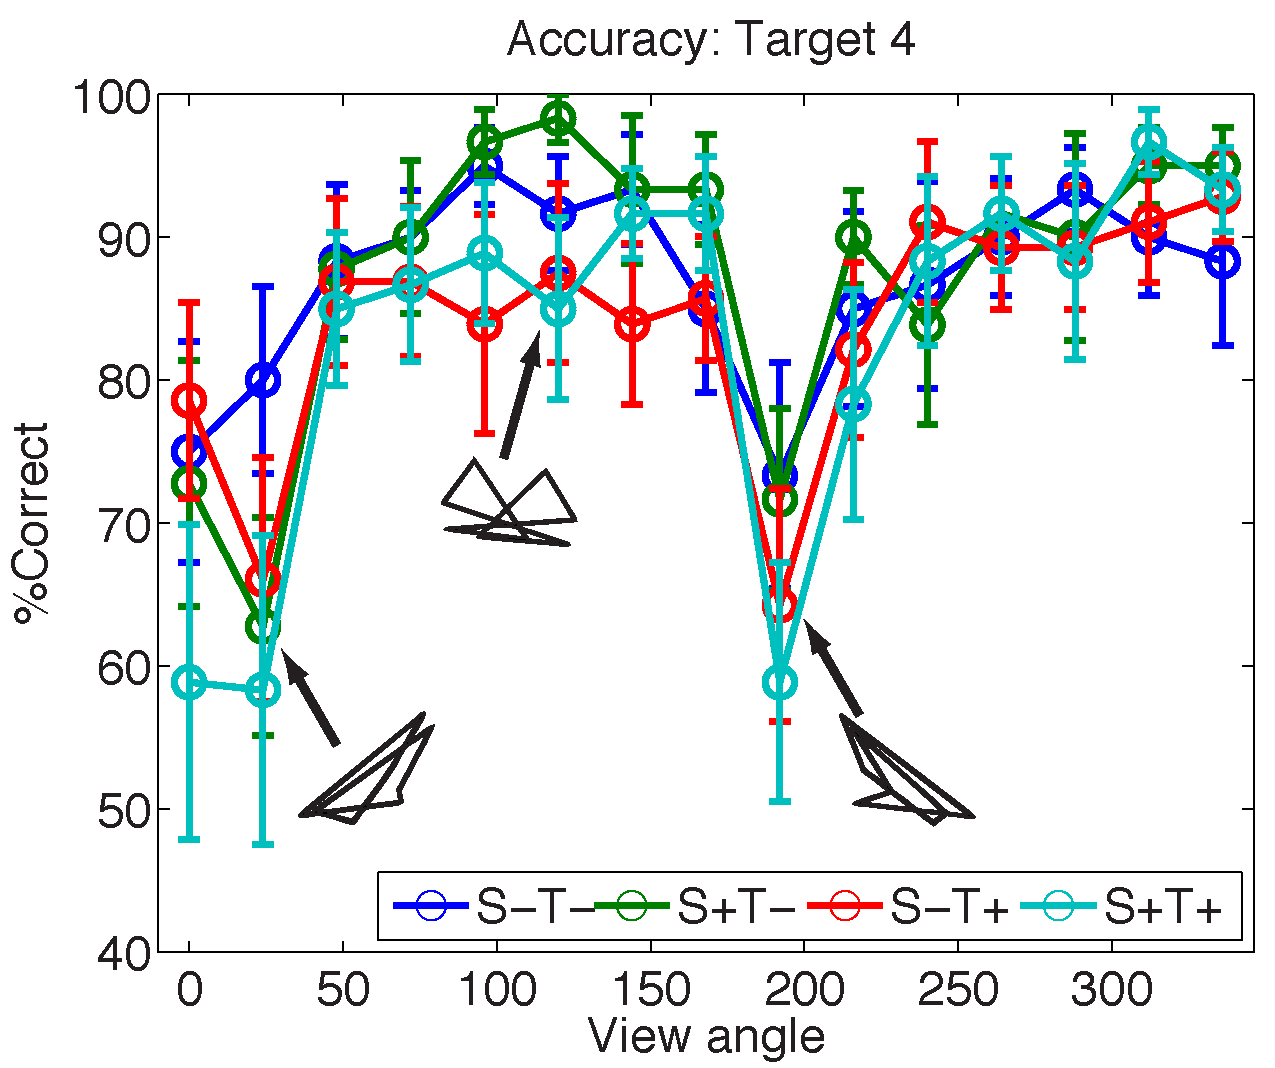
\includegraphics[width=80mm]{figs/chap_bpleast/results_accuracy_rot_obj4_montage.pdf} \\
\end{tabular}
\end{center}
\caption{Accuracy as a function of viewing angle for each target object}{Target accuracy at each viewing angle presented during the test periods. Horizontal axes denote viewing angle and colors predictability during the training period. Error bars depict between-subjects standard error. Diametrically opposed foreshortened views and one canonical view are shown for target object 4.}
\label{fig:bpleast_behave_rot}
\end{figure}

Standard statistical tests did not have enough power to detect differences between conditions for degenerate views due to the low trial counts for each data point. To address this design limitation, a bootstrapping method was used to resample the available data in these cases. The completely unpredictable (S-T-) and combined spatial and temporal predictability (S+T+) were used to assess differences due to training context since these two conditions elicited the greatest difference in average accuracy in the full analysis. The accuracy function over viewing angles was collapsed across conditions and the two minima associated with degenerate views were identified for each object. For target object 1, the two views were at $\theta$ = (24$^\circ$, 312$^\circ$), object 2: $\theta$ = (48$^\circ$, 240$^\circ$), object 3: $\theta$ = (144$^\circ$, 312$^\circ$), and object 4: $\theta$ = (24$^\circ$, 192$^\circ$). S-T- and S+T+ accuracy was averaged at each object's degenerate views and resampled with replacement from the 59 subjects for 10000 iterations. This produced degenerate view accuracy distributions for spatiotemporally unpredictable and predictable training contexts (Figure \ref{fig:bpleast_behave_bootstrap}). Accuracy was lower for degenerate views studied under the spatiotemporally predictable context for all target objects except target 1, which didn't exhibit the patterned accuracy function that other targets did. The predictability difference in accuracy for degenerate views was significant at the 90\% alpha level (i.e., the confidence interval of the difference between means did not include zero) for all target objects except target 1.

% oh, behave, pt 4: bootstraps
\begin{figure}[h!]
\begin{center}
\begin{tabular}{ll}
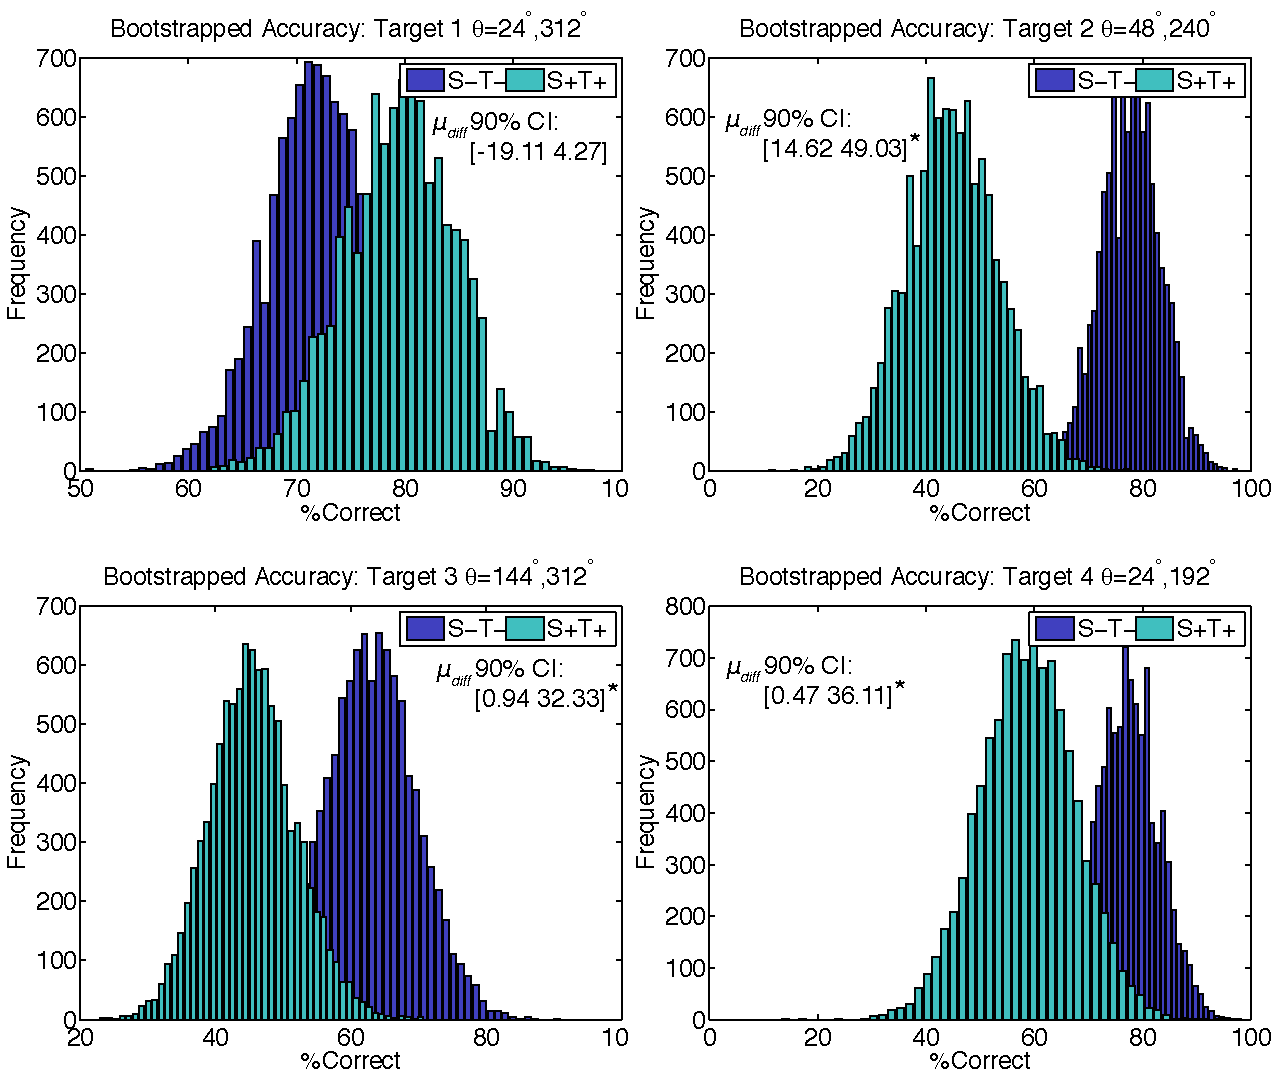
\includegraphics[width=160mm]{figs/chap_bpleast/results_bootstrap_montage.pdf}
\end{tabular}
\end{center}
\caption{Bootstrapped accuracy for degenerate views}{Average target accuracy for degenerate views resampled with replacement from the 59 subjects for 10000 iterations. Viewing angles for averaging is noted for each target object. Asterisks denote significant differences based on 90\% confidence intervals.}
\label{fig:bpleast_behave_bootstrap}
\end{figure}

\section{Discussion}\subsection{Summary of results}
The work described in this chapter investigated how predictability biased representations of novel objects over prolonged learning. The experimental paradigm used to address this question involved training participants to recognize novel objects while manipulating their spatial and temporal predictability. Somewhat surprisingly, accuracy was lowest when stimuli were learned in a combined spatially and temporally predictable context and highest when learned in a completely unpredictable context. Reaction times were also slower when objects were learned with spatial predictability. These findings were unexpected because the spatial structure of the physical world has been suggested to be a powerful learning mechanism when coupled with the putative temporal association rules of visual neurons \cite{StringerPerryRollsEtAl06,WallisBaddeley97,IsikLeiboPoggio12,SakaiMiyashita91,MeyerOlson11,CoxMeierOerteltEtAl05,LiDiCarlo08,LiDiCarlo10,LiDiCarlo12}.

Behavioral measures were highly variable across objects used in the experiment. There was some indication that the principal differences between predictability conditions during training were driven primarily by degenerate viewing angles caused by three-dimensional foreshortening in the objects used. In three out of four objects, accuracy was lower for degenerate views learned in a spatiotemporally predictable context compared to a completely unpredictable one.

\subsection{A behavioral disadvantage for spatial prediction during object learning}
Intuitively, spatial predictability should be advantageous for learning the three-dimensional structure of objects given that it is the learning context within which the visual system evolved. However, the literature contains a mixture of contradictory effects regarding the utility of spatially predictable information during object learning and recognition. Initial experiments described in \incite{LawsonHumphreysWatson94} with depth-rotated line drawings of familiar objects demonstrated the expected increase in recognition accuracy for spatially predictable sequences. A number of studies have found that studying depth-rotating sequences of novel objects under one ordering and then testing with a different ordering impairs recognition \cite{Stone98,VuongTarr04,ChuangVuongBulthoff12}, implying that learned spatial predictability about the sequence is used to encode the object \cite{BalasSinha09c}. The foreshortening model advanced in \cite{BalasSinha09b} also provided a better match to observers' data by incorporating spatial information (e.g., the first- and second-order derivatives of the foreshortening function over object views).

Some of the experiments described in \incite{LawsonHumphreysWatson94}, however, demonstrated better accuracy for sequences studied with weak spatial predictability (maximum of two consecutive spatially coherent frames in a sequence) than total spatial predictability. Experiments described in \incite{HarmanHumphrey99} failed to find any positive or negative effects of spatial predictability on accuracy. They did, however, increase in reaction time for objects learned in a spatially predictable context, similar to the one reported here. 

One possible reason for the behavioral disadvantage for objects learned with spatial predictability is that less attention is necessary in these conditions. A constantly changing sequence of views might require more attentive processing to encode whereas the relatively small amount of change between views in spatially predictable sequences is comparatively ``unsurprising'' such that some views might be overlooked during encoding \cite{TarrGauthier98}. However, there was some indication that the adverse effects of spatial predictability in the current experiment were driven primarily by the degenerate views of particular stimuli. A more focused experiment is clearly necessary to explicitly test the hypothesis that behavioral performance is impaired for degenerate views learned in a spatially predictable context but relatively intact for canonical views. 

\subsection{Building viewpoint invariance for three-dimensional objects}
Given the cumulative literature considered here, the most reasonable interpretation of the experimental results is as follows: Three-dimensional objects are typically represented in a viewpoint-dependent manner \cite{WallisBulthoff99,EdelmanBulthoff92,TarrGauthier98,LogothetisPaulsBulthoffEtAl94,LogothetisPaulsPoggio95}. Each of these views is associated with the given object's identity to the degree to which three-dimensional features are recoverable from the two-dimensional projection. This can lead to low accuracy for degenerate viewing angles caused by extreme three-dimensional foreshortening demonstrated here and in previous studies \cite{BalasSinha09b}. 

When three-dimensional objects are studied in a full spatiotemporally predictable context, temporal association mechanisms are invoked that build viewpoint invariance \cite{CoxMeierOerteltEtAl05,LiDiCarlo08,LiDiCarlo10,LiDiCarlo12}. This invariance accounts for variability due to foreshortening but is actually \textit{not optimal} for three-dimensional objects that need to be recognized from individual static views. If the full spatiotemporal sequence is available when the object needs recognized (as is typical in real world object recognition) accuracy is not impaired by degenerate views and activation of the newly acquired invariant features might even be facilitated \cite{BalasSinha09c}. However, if only static views are available during recognition, or perhaps worse, the full sequence is available but not in its spatially predictable order, it is not possible to activate these invariant features, leading to impaired recognition \cite{Stone98,VuongTarr04,ChuangVuongBulthoff12}.

The corollary of this interpretation is that when three-dimensional objects are studied in a completely unpredictable context, temporal association mechanisms are actually \textit{not invoked}. Further research is needed to determine if this assertion is plausible, and if so, precisely why these mechanisms would not be active. However, one possibility is that temporal associations operate over samples of an input sequence at regular intervals (e.g., 100 ms, see Chapter \ref{chap:leabrati}). When input sequences don't align to these sampling intervals, the associations between subsequent inputs cannot be formed. The result is that despite prolonged learning, the objects remain represented in a viewpoint-dependent manner, which facilitates recognition for static views.

%\bibliographystyle{apa}
%\bibliography{ccnlab}

\end{document}